% !TeX root = ../Thesis.tex
\documentclass[../Thesis.tex]{subfiles}
\graphicspath{{\subfix{../images/}}}

\begin{document}

\section{Compiler architecture}
\label{sec:compiler-architecture}

Compilers are programs that transform source code
written in one language into another language, usually machine code.
A compiler takes in a program in one language, the \emph{source} language,
and translates it into an equivalent program in another language,
the \emph{target} language.

To achieve this, compilers typically have a series of phases or passes
that are executed in sequence.
The goal of these passes is to translate the high-level code
into low-level code that the machine can execute.
In each pass, the code is brought closer and closer to the final representation.
These phases are nowadays well-defined and
different compilers implement some form of them \cite[Chapter 1.2]{aho2014compilers}.

The first pass of a typical compiler is the \textbf{lexical analysis} phase.
In this phase, the source code is broken down into a stream of tokens,
each of which represents a single piece of the code.
The \emph{lexer} identifies keywords, identifiers, literals, and other tokens
that form the building blocks of the source code.

The next pass is the \textbf{syntax analysis} phase, also known as the parser phase.
In this phase, the tokens produced by the lexer are analyzed
according to the rules of the programming language's grammar.
The \emph{parser} constructs a parse tree or an \acrfull{AST}
that represents the structure of the code.

The third pass is the \textbf{semantic analysis} phase,
in which the compiler checks the code for semantic correctness,
such as checking for type errors, undefined variables, and invalid operations.
The \emph{semantic analyzer} builds a symbol table that contains information
about the variables, functions, and other entities defined in the code.

The fourth pass is the \textbf{code generation} phase.
The compiler takes the \acrshort{AST} and symbol table produced by the previous phases
and generates low-level code that can be executed by the machine.
The code generator typically generates code in assembly language or machine code.
In other cases, it generates bytecode,
as in Java or when using the Python \acrfull{JIT} compiler.

Finally, there may be zero or more \textbf{code optimization} phases.
These are from a theoretical point of view optional,
but they are usually included by default in modern compilers.
In this phase, the compiler analyzes the generated code
and attempts to improve its efficiency by applying various optimization techniques.
Some examples of optimizations include:

\begin{itemize}
    \item constant folding \cite[Chapter 8.5.4]{aho2014compilers},
    \item loop unrolling \cite[Chapter 10.5]{aho2014compilers},
    \item register allocation \cite[Chapter 8.1.4]{aho2014compilers},
    \item constant propagation \cite[Chapter 9]{aho2014compilers},
    \item liveness analysis \cite[Chapter 9]{aho2014compilers},
    \item and many more\ldots
\end{itemize}

\emph{Local} code optimizations concern improvements within a basic block,
whereas \emph{global} code optimization is when improvements take into account
what happens across basic blocks.
In Rust, one example of global optimization is \acrfull{LTO} \cite{huss2020}.

Fig. \ref{fig:compiler-phases} taken from \cite{aho2014compilers}
summarizes the compiler phases described in this section.

\begin{figure}[!htb]
    \centering
    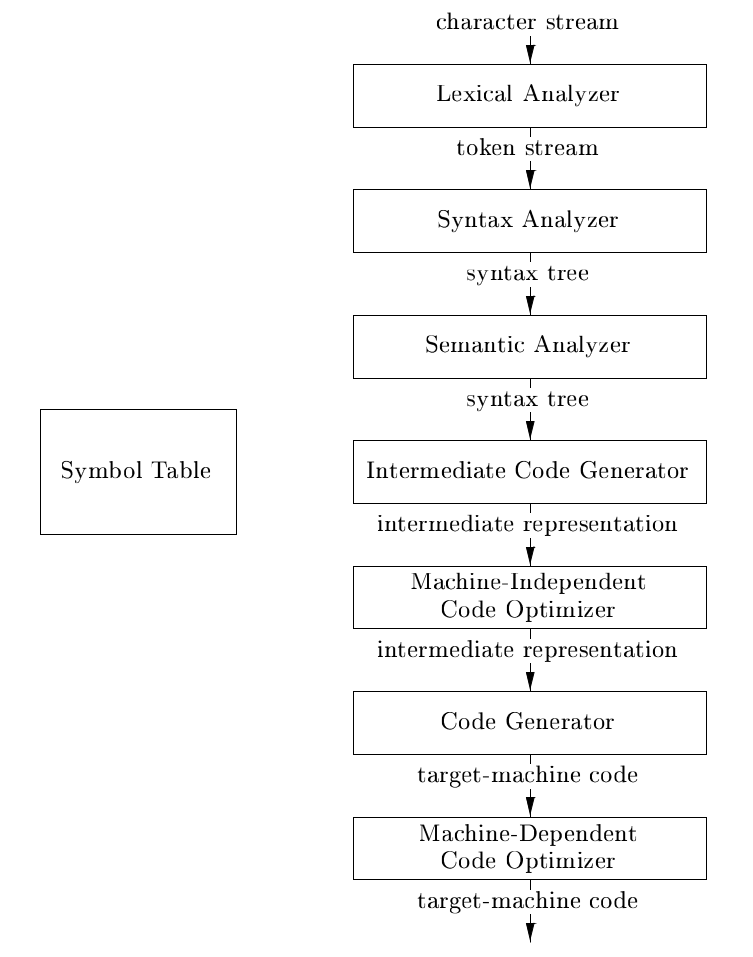
\includegraphics[scale=0.40]{compiler-phases.png}
    \caption{Phases of a compiler}
    \label{fig:compiler-phases}
\end{figure}

In practice, phases might have unclear boundaries.
They can overlap and some may be skipped entirely.
In later sections, we will study the architecture of the Rust compiler \emph{rustc}
and explain its general architecture.

\end{document}